\documentclass[tikz,a4paper,titlepage]{article}
% For Gantt Chart 1 (by month)
\usepackage{pgfgantt}
\usepackage{xcolor}
\usepackage[parfill]{parskip}
\usepackage[utf8x]{inputenc}
\usepackage[english]{babel}
\usepackage[T1]{fontenc}
\usepackage{graphicx}
\usepackage{adjustbox}
\usepackage{float}
\usepackage[final]{pdfpages}
\usepackage{listings}
\usepackage[colorlinks=true, allcolors=blue]{hyperref}
\usepackage[a4paper,top=0.75in,bottom=0.75in,left=0.75in,right=0.75in,marginparwidth=1.75cm]{geometry}
%\usepackage[paper=portrait,pagesize]{typearea}
% \usepackage{lscape}
\usepackage{rotating}
\usepackage{pdflscape}
\graphicspath{{./Images/}}

% For Gantt Chart 2 (by week)
%\usepackage{pgfgantt}
\definecolor{barblue}{RGB}{153,204,254}
\definecolor{groupblue}{RGB}{51,102,254}
\definecolor{linkred}{RGB}{165,0,33}
\renewcommand\sfdefault{phv}
\renewcommand\mddefault{mc}
\renewcommand\bfdefault{bc}
\setganttlinklabel{s-s}{START-TO-START}
\setganttlinklabel{f-s}{FINISH-TO-START}
\setganttlinklabel{f-f}{FINISH-TO-FINISH}
\sffamily

% Colors for Gantt chart:
% Find color schemes using: https://www.w3schools.com/colors/colors_monochromatic.asp

% Blue color scheme
\definecolor{colorone}{RGB}{96,156,225}
\definecolor{colortwo}{RGB}{35,106,185}
\definecolor{colorthree}{RGB}{19,56,99}

% Red color scheme
%\definecolor{colorone}{RGB}{254,143,119}
%\definecolor{colortwo}{RGB}{253,58,15}
%\definecolor{colorthree}{RGB}{167,32,2}

% lstset for setting styles for source code
\lstset{ %
  backgroundcolor=\color{white},   % choose the background color; you must add \usepackage{color} or \usepackage{xcolor}; should come as last argument
  basicstyle=\footnotesize,        % the size of the fonts that are used for the code
  breakatwhitespace=true,         % sets if automatic breaks should only happen at whitespace
  breaklines=true,                 % sets automatic line breaking
  captionpos=b,                    % sets the caption-position to bottom
  commentstyle=\color{blue},    % comment style
  extendedchars=true,              % lets you use non-ASCII characters; for 8-bits encodings only, does not work with UTF-8
  keepspaces=true,                 % keeps spaces in text, useful for keeping indentation of code (possibly needs columns=flexible)
  identifierstyle=\color{purple},
  keywordstyle=\color{orange},       % keyword style
  language=Verilog,                 % the language of the code
  morekeywords={*,char,int,struct,bool},           % if you want to add more keywords to the set
  rulecolor=\color{black},         % if not set, the frame-color may be changed on line-breaks within not-black text (e.g. comments (green here))
  showspaces=false,                % show spaces everywhere adding particular underscores; it overrides 'showstringspaces'
  showstringspaces=false,          % underline spaces within strings only
  showtabs=false,                  % show tabs within strings adding particular underscores
  stepnumber=2,                    % the step between two line-numbers. If it's 1, each line will be numbered
  stringstyle=\color{red},     % string literal style
  tabsize=2,	                   % sets default tabsize to 2 spaces
  title=\lstname                   % show the filename of files included with \lstinputlisting; also try caption instead of title
}


\begin{document}

\begin{titlepage}
\vspace*{\fill}

\newcommand{\HRule}{\rule{\linewidth}{0.5mm}} % Defines a new command for the horizontal lines, change thickness here

\center % Center everything on the page

%----------------------------------------------------------------------------------------
%TITLE SECTION
%----------------------------------------------------------------------------------------

{ \huge \bfseries IoT Security Project Design}\\[0.4cm] % Title of your document

%----------------------------------------------------------------------------------------
%HEADING SECTIONS
%----------------------------------------------------------------------------------------

\textsc{\LARGE Sean Caster, Vincenzo Piscitello, Adam Barton, Ryan Howerton, and Terri Hewitt}\\[0.5cm] % Name of your university/college
\textsc{\Large Senior Design}\\[0.5cm] % Major heading such as course name
\textsc{\large Fall 2018}\\[2.5cm] % Minor heading such as course title


%\HRule \\[0.8cm]
\begin{minipage}{0.8\textwidth}  % Set width of abstract
%\HRule \\[0.8cm]
\textbf{\large Abstract} \\
\HRule \\[0.4cm]
The goal of this project will be to implement a secured, decentralized meshnet with low minimum resource requirements to enable the connection of a wide variety of low-end devices which lack a general purpose operating system. Our objective will be to investigate the amount of security offered and resources required by various cryptosystems in order to provide organizations interested in securing their low-end device networks with a quantified estimate of the costs and benefits. In addition, we hope to accomplish graceful degradation on our network, meaning that the elimination or temporary unavailability of a given node will have minimal negative impact on the inter-connectivity of other nodes. This will encourage the securing of many resource limited devices which play a critical role in meeting a wide variety of human needs.
\\[0.4cm]
\HRule \\[1.5cm]
\end{minipage}
%\HRule \\[1.5cm]

                %----------------------------------------------------------------------------------------
                %DATE SECTION
                %-----------------    -----------------------------------------------------------------------

{\large November 27, 2018}\\[3cm] % Date, change the \today to a set date if you want to be precise

%----------------------------------------------------------------------------------------
%LOGO SECTION
%------   ----------------------------------------------------------------------------------

%
\includegraphics{Logo}\\[1cm] % Include a department/university logo - this will require the graphicx package

%----------------------------------------------------------------------------------------

\vfill % Fill the rest of the page with whitespace

\end{titlepage}

\tableofcontents
\newpage

\section{Scope}

The ultimate goal of this project will be to produce the implementation and verification of the secure networking paradigm succinctly named Brypt. Brypt combines the main cornerstones of the software, bridging and encrypting. The implementation will provide a central server, binaries for node endpoints, and a security protocol working on top of the session layer. In completing the work on this project our team aims to provide a novel solution to security in interconnected networks of embedded and general purpose devices. Some of the benefits Brypt will provide include the increased viability of secure cryptographic primitives in power constrained environments across a number of different communication technologies. 

As it stands, a wide variety of mission critical tasks for many utility grids (water, power, etc.) are accomplished by low power embedded devices. The mass quantity of devices required to fulfill the operational needs of these networks has created a systemic problem of sacrificing security to reduce the cost of power. The purpose of our system, Brypt, will aim to provide a solution for architects of these networks to have the best of both worlds. In minimizing the cost of power while maximizing the security of ad-hoc mesh networks will demonstrate numerous benefits.

In addition to offering an implementation of what our investigations suggest to be an excellent general purpose meshnet cryptosystem, we will generate useful data about the costs of resource asymmetric cryptosystems that can be applied to the design of more special purpose meshnets by organizations looking to secure their particular resource distribution optimally. These findings will be published in a final report alongside the implemented network to help in the potential design of such future projects.

\section{Stakeholders}

\subsection{Internal Stakeholders}

All members of the IoT Security Research team and our client, Kevin McGrath, who is in association with McAfee and Oregon State University, hold an interest in the results of this research.

% Anyone have design concerns??

\subsection{External Stakeholders}

The results of this research project will be of interest/concern to members of the IoT development community, IoT industries (i.e. smart devices and utility grids), and consumers of those products. 


% Just us and Kevin...I think?
%TODO: \\
%An SDD shall identify the design stakeholders for the design subject.
%An SDD shall identify the design concerns of each identified design stakeholder.
%An SDD shall address each identified design concern. 

\section{References}

\begingroup
\renewcommand{\section}[2]{}%
%\renewcommand{\chapter}[2]{}% for other classes
\bibliographystyle{ieeetr}
\bibliography{citations}
\endgroup 

\section{Context}

From smart-grids to autonomous cars to needlessly elaborate refrigerators, the use of embedded devices and the size of the IoT is one of the fastest growing areas of computation in our time. With this growth comes the unique challenge of implementing security on highly cost-prohibitive devices. Though much arduous work has already been put into optimizing resource usage of cryptosystems, the highly resource asymmetric nature of many of these IoT network topologies leaves room for more bespoke optimization strategies which take into consideration the resource distribution of the network. In this new context, doubling the \textit{overall} computation used by a cryptosystem may actually be an improvement, so long as the computation required of the weakest devices on the network decreases adequately (since in many circumstances an increase in server power may be 25\% as expensive as a comparable increase in embedded device power on the same network). In order to help organizations enumerate the cost of securing their embedded device networks, we aim to provide real world, experimental data about the electricity and computation usage of a myriad of cryptosystems, some of which will be designed with resource asymmetry in mind. 

Brypt will not only provide the secure network created to our stakeholders, but also research done on the network to investigate power consumption and security trade-offs. One service this project provides is information on implementation of this secure mesh network in distinct environments. This implementation will span three communication protocols with varying wireless ranges using a mesh-network designed for a wide range of real world potential uses. However, most stakeholders may want to simply interact with our project. These stakeholders can interact through our three provided interfaces discussed in section \ref{server_api}. These interfaces include a home-page providing information and binaries for these users to implement on their own. In addition, this interface provides the ability for users to register and log in. Lastly, users can interact to the system through the dashboard to manage their cluster-networks as well as to authenticate new nodes onto their cluster network. Some of our stakeholders such as members of the IoT industry may not be as interested in the specific implementation of our network or how to implement it themselves, but are more interested in the outcome of our research. These stakeholders will be able to view our research on our network as to the trade-offs between security, power consumption, and see how feasible it is to implement security on low-power embedded devices.

\section{Implementation}

\subsection{Server API} % Design View
\label{server_api}

The Central Server of the Brypt Architecture will serve two purposes within the context of our system.

The first responsibility of the server is that of serving web application pages and the handling of communications with a client computer. A client computer is defined as being any general purpose computer with internet connectivity and a modern browser. These application pages will be served dynamically through three discrete routers deployed under the single Brypt domain. These three interfaces provided by our web application are broken into three logically separated subdomains due to the distinct functionalities provided. The first interface provided by the central server will handle requests with all visitors from our front facing web-page. The front-facing web interface to be serviced by the www.brypt.com subdomain will present basic information about the Brypt system as well as the ability to download Brypt binaries. These binaries will enable any computer with internet access to operate as a cluster node on a Brypt network. The second interface served by the Brypt server will be the web-based application dashboard. This dashboard will handle the management of a user’s network clusters and parse data transmissions from their network. The dashboard interface will be accessible through the dashboard.brypt.com subdomain. Our third interface and that which serves as an intermediary to the two previously discussed interfaces is the access portal. This access interface serviced by access.brypt.com will provide user registration and login functionalities.

The second responsibility of our central server will be the authentication and authorization of nodes and joining nodes to the network. The bridge.brypt.com subdomain will provide node administration services. This server endpoint will have an associated user interface accessible through the dashboard application. This interface will request the UUID of the node which in turn tells the server to listen for connections from that device. Upon contact from the node, the server will provide the device a pre-image puzzle based on a unique identifier specific to the node. Once this puzzle has successfully been solved the node will be considered authenticated and provided network connection information.

In order to provide the desired functionalities as fast and as efficient as possible the central server will be written using the Go programming language. Go will enable our team the ability to develop each subdomain router individually and as a distinct package while maintaining a method of interconnection between them. The structure of Brypt server will be based on the REST architecture and as such we will be handling all requests using HTTP/S. We will be utilizing the Go-Chi library to act as a lightweight request handler for our server. To ensure the maximum amount of security in client-server communications our server will ensure all HTTP requests are redirected to the appropriate HTTPS url.

\subsection{Database Design}

The Brypt system will require a database to maintain persistent data storage for users, networks, and node information within the ecosystem. As we anticipate the need for flexibility and large collections we have chosen MongoDB as our database driver. MongoDB will provide our desired requirements through its use of a JSON like structure, known as BSON, and sharding capabilities. BSON documents within MongoDB will allow fields to be dropped-in and out fields as the schema requires as well as elegant sharding as our collections grow. If access to Brypt’s data based on location is needed, MongoDB has the built-in ability to shard collections based on geolocation. The database will be organized into three document collections: Users, Networks, and Nodes. The Users collection will store documents for each individual registered through the web application. A user document will contain contact information, login credentials, associated networks, and other user-specific data. The Networks collection will maintain a document for independent user networks operating on the Brypt architecture. A network document will store network usage information, network credentials, network owners and managers, and associated cluster coordinators within the network. The final collection, Nodes, will maintain a list of all authorized nodes which are generated by flashed embedded devices or the installation of the Brypt binary on a general purpose computer. A node document contains identifiable information about the device. The database itself will be encrypted for secure storage as well as using an encrypted connection from an account with appropriate permissions for data transmission and management.

% Any subsubsections should be Design Viewpoints (see https://ieeexplore.ieee.org/stamp/stamp.jsp?tp=&arnumber=5167255)

% Mention any Design Relationships the Server API has with any other design viewpoints or views

\subsection{Web Application}

The primary interface of our system will be provided through a cloud based application served through our central server. Within our web application three primary access points will be available to the user. The first interface will be the base information page for Brypt; this page will contain information about the system, it’s requirements, and downloads. The second interface will be the node management screen; these pages will provide node network authorization. The final user interface element of our system is the dashboard page which will contain information pertaining to the status of the user’s connected clusters and aggregation of the nodal data. The only requirement of the user will be access to a browser capable device. Outside of our application interface, users will need to interact with our embedded devices and/or binaries for their system of choice. The frontend of our web application will be serviced through the utilization of HTML, CSS, JavaScript, and Vue.js. Each page to be served will be templated and compiled server side which will then be handled by Vue.js for client side interaction and AJAX communications. 

\subsection{Node Networking}

The network as a whole will be broken down into sub-networks based on the communication protocol used between devices. One root network consisting of a root network coordinator and the multi-communication protocol capable network coordinator nodes. This network will provide aggregated data in packets to be sent to the web-application and central server. These powerful nodes within the root network will act as coordinators of a sub-network for a specific communication protocol type (see Figure \ref{fig:isn}).


\begin{figure}[h]
  \centering
    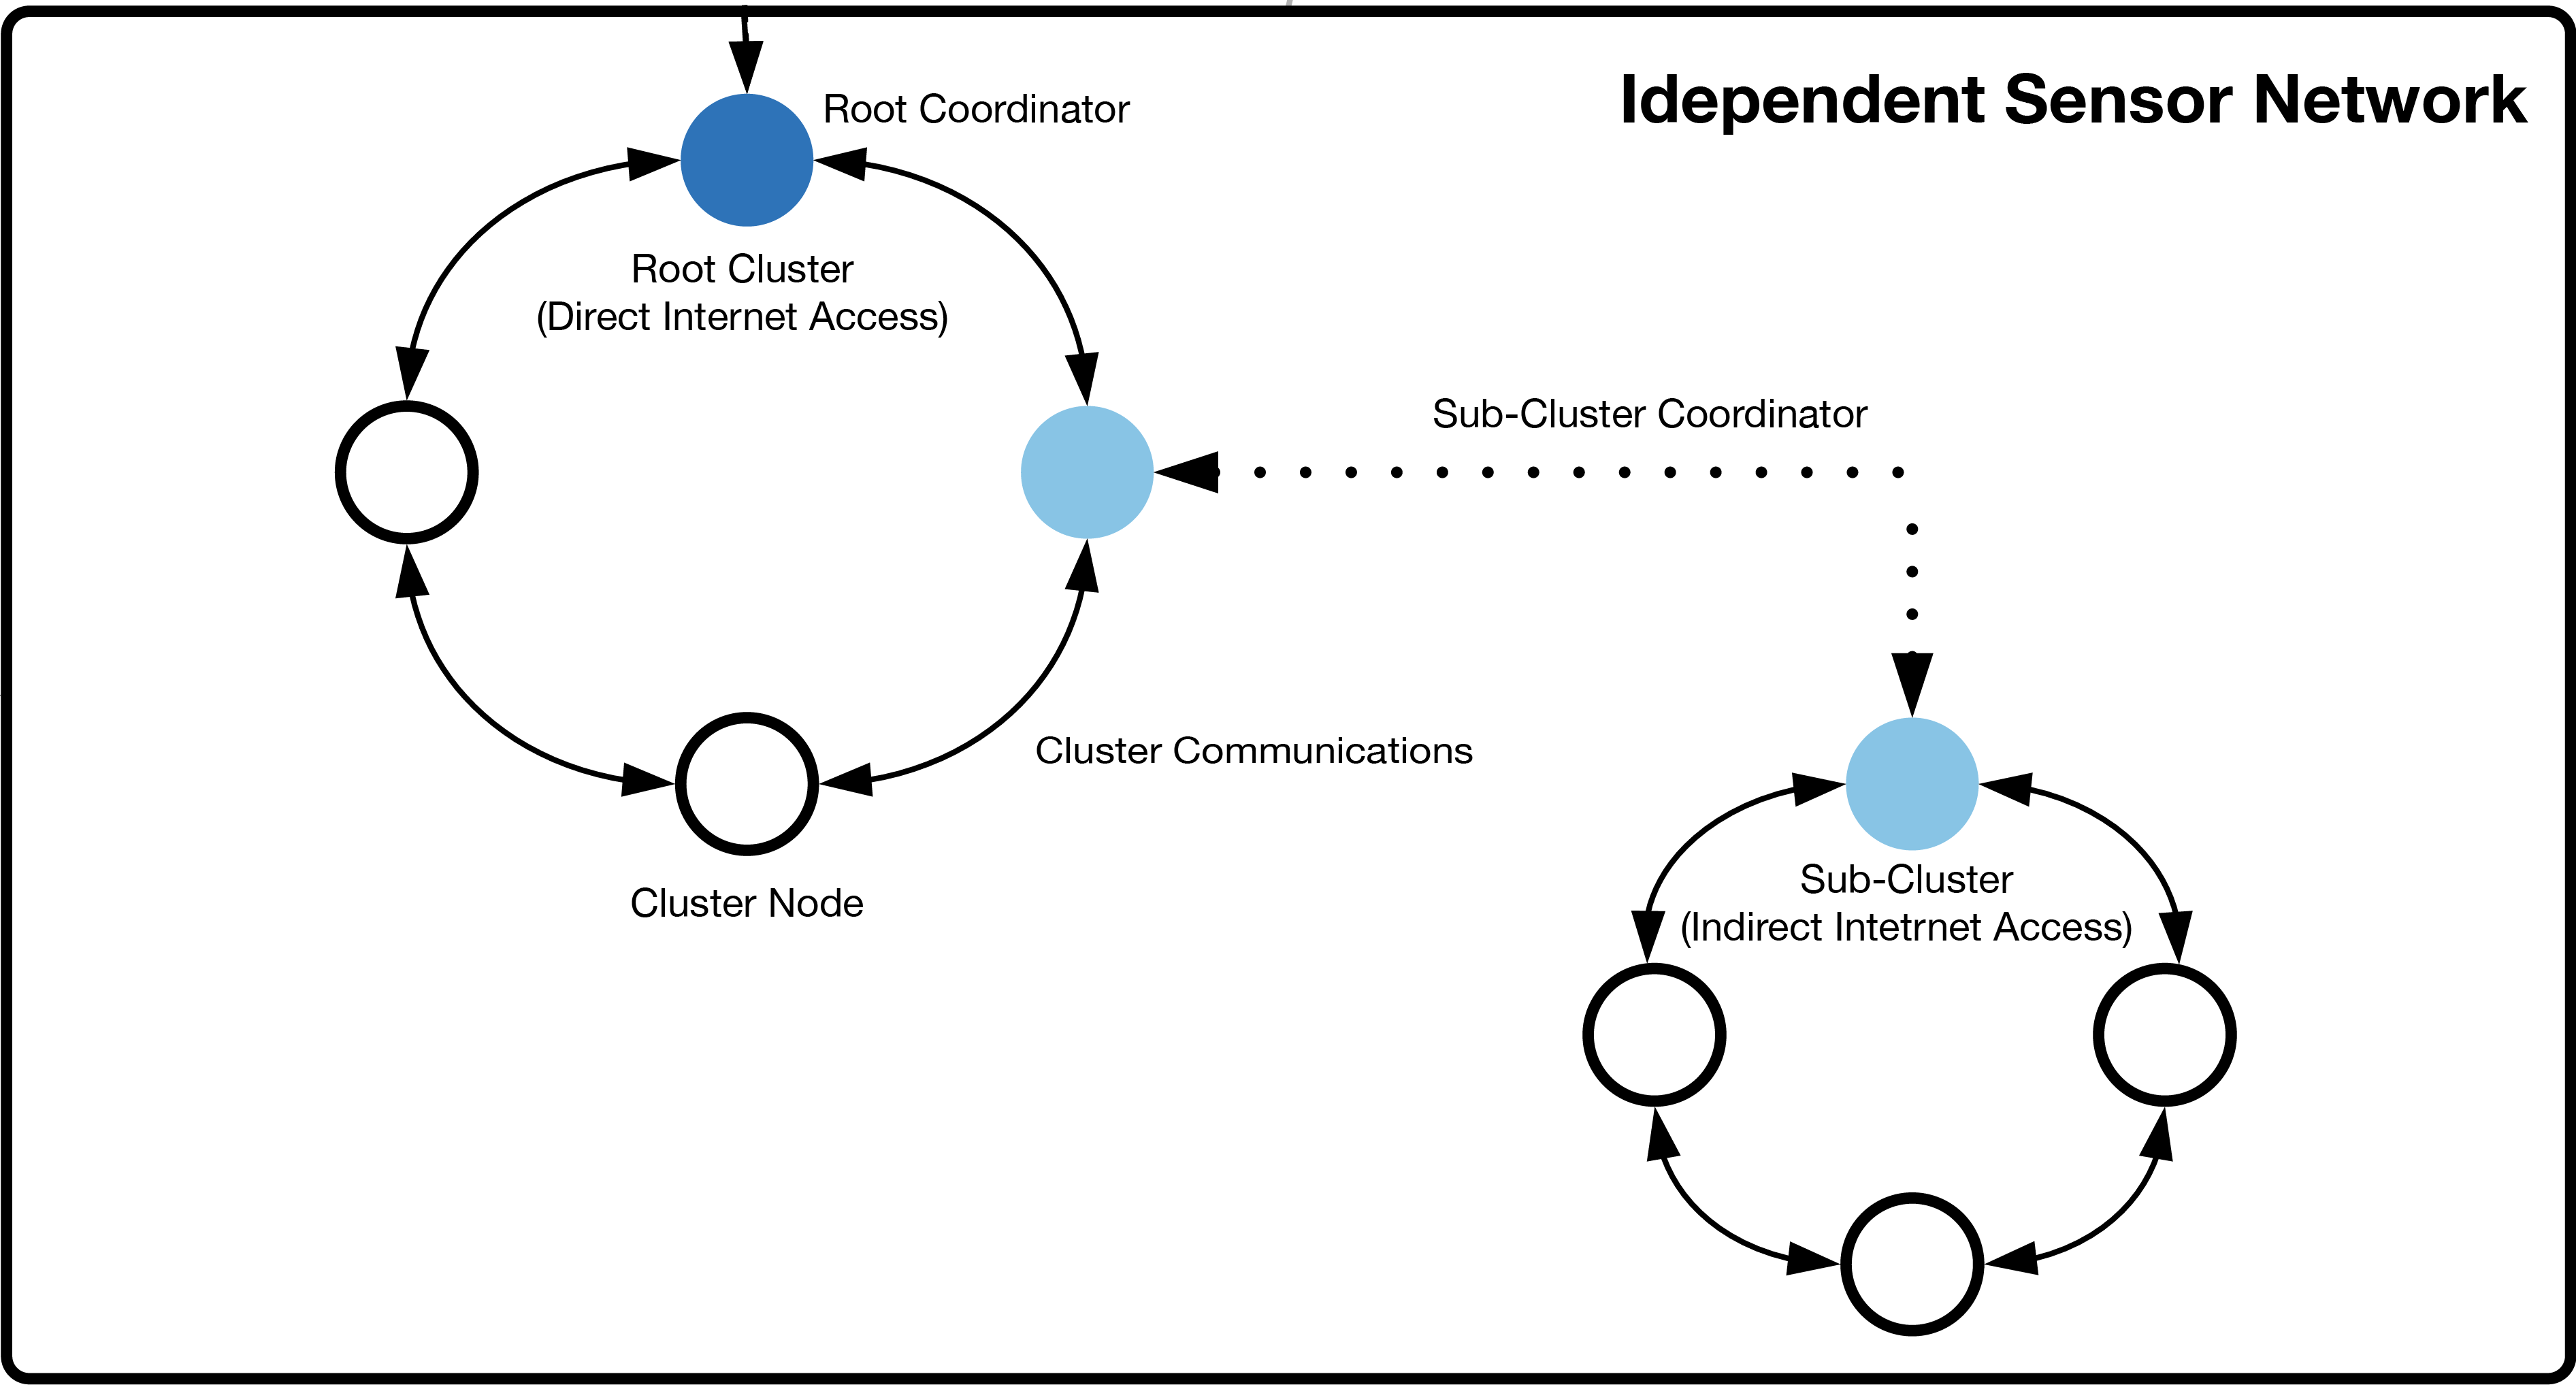
\includegraphics[width=.9\linewidth]{Images/draft-brypt-architecture-isn.png}
  \caption{Organization of root and sub-cluster networks}
  \label{fig:isn}
\end{figure}


To begin, we will need to implement a pseudo-mesh network which will be used as the platform for our research on the financial and computational costs of securing a node. The implementation of our base network will be composed of a central routing authority and low power nodes. The central routing authority will operate on a remote server which will perform verification and authorization of the network nodes. The mode of authentication will use an aggregate or sequential encryption puzzle (see section \ref{node_auth}) to verify the potential network node while also providing some level of DDOS protection. The central server interface will request the nodes UUID as input and listen for the individual node to make contact. Upon first contact to node will compute a encryption puzzle based on their production key provided from installation.

After a node has successfully solved the check it will be provided routing information to a coordinator node for its specific communication protocol. If the network has separate clusters and the user has requested to join a specific group, that information will be provided to the new node for routing. Given that the node network will be developed based on a multi-hop mesh network, the new node will perform a series of acknowledgements to be configured into the topology. During this configuration process the node will generate a transmission “line” table to be able to communicate with as many peers it has access too. Utilizing the information of it’s cluster the node will be able to perform it’s base operation and listen for failed peers. If a peer has failed it’s security check, as it has been compromised or has gone offline, the coordinator will be notified and the network will reconfigure.

The web-application will be integrated into the network either as a node or through the central server and will generate queries for the networked devices. Queries will be routed through a network graph structure to embedded devices. Messages will propagate through the graph from these devices to reach the web-application.

% -Root coordinator in network of coordinators
% -Node tree structure (topology)


\subsubsection{Communication Technologies}

% WiFi, LoRa, BLE - how we're going to implement this on all of the network devices
Devices in the network will be able to communicate on one of three different technologies: Wi-Fi, LoRa, or Bluetooth. The devices used for this network as nodes will be Adafruit Featherboards, while Raspberry Pi computers will act as network coordinators. We chose these devices because they have differing architectures and capabilities, and so will better simulate an actual IoT network: the Featherboards will be chosen from BLE, LoRa, and ARM Cortex Wi-Fi and ESP-8266 Wi-Fi. Coordinator nodes will have receivers and transmitters for all three types so that they can fulfill their duty of translating between the radio types. The root network will contain the coordinator nodes for the sub-networks and will communicate over Wi-Fi.

\subsubsection{Communication Protocols}

The database will contain a collection of every node in the network, stored with their assigned addresses (assigned by the coordinators). Each coordinator will store a table of every node in its direct cluster, again with their assigned address. This table can include other coordinators that will control smaller groups of nodes that potentially operate with a different radio technology. Additionally, each node will have a similar, smaller table that contains all nodes that are within their communication range that they are able to communicate with. Thus, our network structure can be described by an undirected graph.

When the Client makes a request to the network, the request is first passed to the root coordinator. If that subnet is not the one being queried, the root coordinator will pass the request to the proper coordinator in its list, and so on until the request reaches the target cluster. At that point, the query is given to all nodes in the cluster. If a node does not have direct communication with the coordinator, other nodes will pass along the query. Once all nodes are aware of the query, they record their data and pass it up the chain, concatenating their own recordings into the packet, until it reaches the coordinator where it will be processed and signed and passed up to the Client. The packet as mentioned, after having been signed will have the following structure: \\

\begin{lstlisting}
{
    coordinator_id: ##,
    node_data: [(node_id: 1, node_data: "..."),
                (node_id: 2, node_data: "..."),
                ...,
                (node_id: N, node_data: "...")],
    packet_signature: "..."
}
\end{lstlisting}
\subsubsection{Verification}

Verification of network connectivity will be through a series of tests. This network provides connectivity between multiple communication protocols and graceful degradation with low minimum resource requirements. Each aspect of the network's abilities will be tested: adding nodes into the network, removing nodes from the network, and message propagation and interface. The interface for our network will allow us to see the outcome of each of these series' of tests. An initial phase of development to provide a proof-of-concept with a working network will be done. After this phase has been verified and tested, development will move onward with security. For our approach to verifying our network's security, see section \ref{net_sec_veri}


\subsection{Research}

% How are we going to conduct our research?
\subsubsection{Phases}

Our research will be conducted in phases. In each phase, the number of CPU cycles and power consumption for each node in our network will be measured as a request for the device's internal temperature is sent from the web application to each node in the network. These measurements will be defined as the cost. The encrypted responses from each node will propagate up to the node's coordinator which will send an aggregated response back to the application. 

For the preliminary phase, Phase 0, no security will be implemented in the network. This phase will act as our control in order to evaluate the added costs of implementing security over the network.

Phase 1 will start with a basic network security implementation. In Phase 1, the first key exchange, performed between a new node entering the network and its coordinator node, any further (general) key exchanges done within each subnet of nodes, will use the RSA protocol. The data field in each network packet will signed using the RSA signature scheme and then encrypted using 3DES at the application layer before being sent through the network. Note that for simplicity, the packet headers will not be encrypted, so it will be possible to trace a message back to its source.

Phase 2 will start integrating Diffie-Hellman key exchange into the basic network security implementation in order to start examining the costs of this key exchange protocol. For Phase 2, the first key exchange and any further key exchanges done will be done using the Diffie-Hellman Key Exchange protocol. The data field in each network packet will signed using the RSA signature scheme and then encrypted using 3DES at the application layer before being sent through the network.

Phase 3 will continue using Diffie-Hellman for the first key exchange, but all other key exchanges will use the AES-CTR "bootstrap" chaining protocol to generate and exchange new keys. Messages will be signed using HMAC with SHA-2 and encrypted with AES-CTR. This phase will be a step up in terms of security as 3DES will be replaced with a more secure cipher: AES-CTR. 

In Phase 4, the first key exchange will use a more costly but also more secure protocol: Elliptic Curve Diffie-Hellman. All further key exchanges will be handled by the node coordinators using the Iolus Group Key Management protocol. Messages will be signed using HMAC with BLAKE2, which is a particularly fast signing algorithm, and encrypted using AES-CTR. This phase is designed to evaluate other strong cryptographic schemes which will likely be more costly than the previous phases.

Lastly, Phase 5 will look at using the RSA public key infrastructure for the first key exchange in combination with Iolus Group Key Management for all other key exchanges. Phase 5 will continue to use AES-CTR for message encryption, but will switch to using FAAS with BLAKE2 to in order to evaluate any reduction in cost associated with using this faster and more efficient aggregate signing protocol. 

% Insert image of network structure

\begin{table*}[h]
\centering
\begin{tabular}{|l|l|l|l|l|}
\hline
        & First Key Exchange & General Key Exchange & Cipher & Signatures \\ \hline
Phase 0 & - & - & - & - \\ \hline
Phase 1 & RSA & RSA & 3DES & RSA \\ \hline
Phase 2 & Diffie-Hellman & Diffie-Hellman & 3DES & RSA \\ \hline
Phase 3 & Diffie-Hellman & AES-CTR Bootstrap & AES-CTR & HMAC (SHA-2) \\ \hline
Phase 4 & Elliptic Curve Diffie-Hellman & Iolus Group Key Management & AES-CTR & HMAC (BLAKE2) \\ \hline
Phase 5 & RSA & Iolus Group Key Management & AES-CTR & FAAS (BLAKE2) \\ \hline
\end{tabular}

\caption{Network security protocols for each phase.}
\label{ResearchPhases}
\end{table*}

If time permits, further research may be done into Post-Quantum (PQ) Lattice cryptography schemes. Phase 6 will attempt to integrate a Post-Quantum Lattice key exchange protocol into the first key exchange to improve the overall security of Phase 5. Phase 7 will then attempt to integrate Post-Quantum cryptography into the message signature and encryption schemes.

\begin{table*}[h]
\centering
\begin{tabular}{|l|l|l|l|l|}
\hline
        & First Key Exchange & General Key Exchange & Cipher & Signatures \\ \hline
Phase 6 & PQ Lattice & Iolus Group Key Management & AES-CTR & FAAS (BLAKE2) \\ \hline
Phase 7 & PQ Lattice & Iolus Group Key Management & PQ cipher & FAAS (PQ hash) \\ \hline
\end{tabular}

\caption{Post-Quantum cryptography stretch goal phases.}
\label{PQ-stretchGoals}
\end{table*}

\subsubsection{Phase Evaluation}

In order to measure the resource usage data collected for each of the cryptosystems planned, our group will be using a combination of an electricity usage measuring voltage meter connected to the power intake of our transmission devices and software tracking for computational resource usage. Time, energy, and expertise permitting, we may look to improve the precision and accuracy of the measurement of our computation resource usage by modifying the CPU schedulers of our devices to handle the tracking of our security-related computation usage.

\subsection{Network Security}

% What security do we plan to implement over the network?

\subsubsection{Node Authentication}
\label{node_auth}



% How we're getting a node on the network. Maybe also how we're authenticating afterward?

Before exchanging keys over the network, nodes and the server will need to ensure they're talking to the computers they intend to. For this reason, each will have to independently authenticate the identity of the other. Though more robust networks use a combination of Public Key Infrastructures and asymmetric cryptography, for now we plan for ours to solve this base authentication problem with pre-flashed fingerprints/public keys for our devices. The exact nature of these fingerprints will vary depending upon the key exchange methodology being used in a given phase as follows.
\begin{itemize}
    \item Modified Diffie-Hellman Key Exchange (DHK) Algorithm
    
    In order to perform authentication during key exchange in a manner that would mimic the costs of PKI usage (which is largely based around use of hash functions for signatures) we'll be flashing the hashes of the expected intermediary keys for Diffie Hellman. I.e. if the node is to send $g^n \%p$ the server will be flashed with hash($g^n\%p$) beforehand, and check that the hash of the key component purportedly from the node matches the pre-stored value. Similarly, if the server is sending $g^s \%p$, the node will be flashed with hash($g^s \%p$) and check the hash of the other key component.
    \item Modified Elliptic-Curve Diffie Hellman Key Exchange (ECDHK) Algorithm
    
    This fingerprinting will work similar to the above: if the node is to send some n*(an elliptic curve P), the server will store hash(n*P). Similarly, if the server is to send some s*P, the node will store hash(s*P).
    \item RSA Algorithm
    
    The fingerprinting for this key exchange will prove comparatively simple. If a server is to use public/private key pair (eS, dS) and a node is to use (eN, dN), the server will be pre-loaded with (eS, dS) and eN, and the node will be flashed with (eN, dN) and eS. From here, a secure encrypted channel can be used to exchange symmetric keys, since authenticity is guaranteed for any node holding dS or dN.
    
\end{itemize}

In addition to authenticating identity during key exchange, our network will also be concerned with ensuring authenticity and integrity of messages encrypted with our normal, bootstrapped symmetric keys. We'll accomplish all enforcement of integrity by universally using the Encrypt then Authenticate standard, meaning that any bits flipped (by adversary or nature) will cause failure of authentication which will cause resending of the message. We'll accomplish authentication with RSA, SHA-2 HMAC, BLAKE2 HMAC, or FAAS with BLAKE-2 depending on the phase. 

\subsubsection{Secure Transmissions and Message Integrity}

% Written in C++??
Once a node is authenticated by the server, the server and node agree on a symmetric key and the node is placed in a subnet based on its communication technology (Wi-Fi, LoRa, or Bluetooth). When the web application requests data from the nodes in each subnet, each individual node will use the given cipher for that phase (either 3DES or AES-CTR) to encrypt the message data at the application layer using the agreed upon symmetric key. However, before the node tranmits its individual response, it must also sign the message using the specified signature scheme for that phase: RSA, HMAC (SHA-2), HMAC (BLAKE2), or FAAS (BLAKE2). Any message signing will be done before the message is encrypted.

The node will then use its routing table to route its response to the next node. Nodes within each subnet will act as routers and forward the packets from other nodes to the next node in the network until the packet reaches the coordinator. When the coordinator collects the responses from all the nodes in its subnet, it will then aggregate the received responses from the nodes in its subnet and then send one aggregated response back to the web application. In the case where at least one of the nodes does not respond to the request, the coordinator will set a timeout starting from when it received the first message from a node. This timeout may vary depending on the normal latency of each subnet, but should initially be set to 5 seconds.

\subsubsection{Threat Response}

% How will our network respond to specific threats (DOS)

\begin{itemize}
    \item Local Watchdog Timers
    
    The purpose of a local watchdog timer is to ensure that runaway computations from faulty or malicious algorithms don't permanently disable a device. They work by periodically scheduling CPU time and sending a signal if the scheduled work is not accomplished in a given time frame. If this signal is sent to the device, it immediately reboots itself in the hopes that whatever problematic state causing interruption of normal CPU scheduling will be an issue in volatile memory that gets reset upon reboot. Though it's not impossible for a problem-state to persist through reboot, the vast majority don't, so it seriously mitigates the physical maintenance requirements of the network its device is running on. These will be active on every node in our network (both the embedded nodes and the coordinators).
    \item Network Watchdog Timers
    
    Though most commonly found on local devices, the principal of a watchdog timer can be applied to network communications as well. By instantiating the server with a maximum amount of appropriate time between messages from a given node, we can detect network abnormalities on the server-side with a good amount of precision (since the server will be able to individually ping every node along the route between it and the non-reporting node). We intend to implement a system where a node exceeding this maximum appropriate radio-silence will be pinged by the server and given an adjustable amount of time to respond (for our purposes likely ~5 seconds). If the device does \textit{not} respond within this timeframe, the server will raise a flag to inform our theoretical network admin of the irregularity. It should be noted here that this provides some new attack surface to our adversary. By implementing this expected behavior, an adversary will have an easy time raising these flags by simply jamming connections. That being said, they'll have to alert authorities of network irregularity in order to do so, so unless they can accomplish something pretty meaningful in the process, it won't necessarily be to their advantage.
    \item Flagging/Graylisting
    
    In addition to tracking the regular communication with nodes, our server will also track the frequency of irregular behavior by the nodes. Things like failed signatures, high latencies, and high packet loss rates will be tracked by the server so it can "score" the overall irregularity of each node's behavior. The benefits of this feature will be two-fold: firstly, many malicious actors will hopefully end up with a high irregularity score, since attacks such as padding oracles require high rates of failed signatures and DoS attacks require creation of high latencies and packet loss. Secondly, it will provide network administrators with data to make more informed, pre-meditated decisions about what hardware needs to be repaired, replaced, or upgraded, since hardware degradation will also drive this irregularity score up. Thus, the increased cost in the interest of the benefit of security may also save auxiliary costs such as overnight shipping and premium hardware prices due to last minute purchases.
\end{itemize}

\subsubsection{Verification}
\label{net_sec_veri}

Though decreasing the electricity and computation required to run a cryptosystem is good, it's only valuable if the newly optimized system is still actually doing its job. In order to confirm this, our group perform penetration testing on our network after each phase is up and running on the network. Though much of this testing will be left free-form to encourage thought about unique properties of each cryptosystem that may be exploitable, we will generally be focusing on the efficacy of PitM and DoS attacks upon each of our implementations. In addition to performing this hollistic analysis, we'll also be projecting the theoretical bit-security of our cryptosystems, so as to be clear about which adversaries the system is actually going to be effective against (i.e. if your adversary model includes nation-states, you'd better have more than 50-bit security).

% What are our plans to verify that everything is working? SEAN: I think we took care if this in verification sections, so I'm commenting this part out

%-Verify our network is working
%-Verify the messages being sent are correct
%-Write about our methods for collecting data (power consumption and computational work)

\section{Summary}

% Summary of our project. What it'll look like in the end.
By the end of this project a secured, decentralized meshnet with low minimum resource requirements will be built. This network will allow for connection from a wide variety of low-end devices which lack a general purpose operating system. Additionally, we hope to accomplish graceful degradation in our network meaning that the elimination or temporary unavailability of a given node will have minimal negative impact on the inter-communication of the other nodes. Most importantly, this network will provide a platform to investigate the amount of security offered by various cryptosystems versus the power costs. Combinations of cryptosystems in "phases" will be implemented across the network and evaluated by their power consumption and security offerings.

\section{Project Timeline}

\begin{ganttchart}[
    x unit=1.1cm,
    y unit title=0.5cm,
    y unit chart=0.6cm,
    vgrid,
    time slot format=isodate-yearmonth,
    compress calendar,
    title/.append style={draw=none, fill=colorone},
    title label font=\sffamily\bfseries\color{white},
    title label node/.append style={below=-1.6ex},
    title left shift=.05,
    title right shift=-.05,
    title height=1,
    bar/.append style={draw=none, fill=colortwo},
    bar height=.6,
    bar label font=\normalsize\color{black!50},
    group right shift=0,
    group top shift=.6,
    group height=.3,
    group peaks height=.2,
    bar incomplete/.append style={fill=colorthree}
   ]{2018-09}{2019-5}
   \gantttitlecalendar{year}\\
   \gantttitlelist{9,10,11,12,1,2,3,4,5}{1} \\
   %\ganttbar[
%    progress=100,
 %   bar progress label font=\small\color{colorone},
 %   bar progress label node/.append style={right=4pt},
 %   bar label font=\normalsize\color{colorone},
 %   name=pp
 %  ]{Preliminary Project}{2018-09}{2018-12} \\
\ganttset{progress label text={}, link/.style={black, -to}}

% Objective 1
\ganttgroup{Server API}{2018-10}{2018-11} \\
% Task A - Start of Jan to end of Jan (1 month)
\ganttbar[progress=50, name=T1A]{Develop Server API}{2018-10}{2018-11} \\
% Task B - Start of Feb to end of Apr (3 months)
% \ganttlinkedbar[progress=0]{Task B}{2019-02}{2019-04} \\
% Task C
% \ganttlinkedbar[progress=0]{Task C}{2019-05}{2019-06} \\

% Objective 2
\ganttgroup{Web Application UI}{2018-11}{2018-12} \\
% Task A
\ganttbar[progress=15, name=T2A]{Develop UI and integrate into server}{2018-11}{2018-12} \\
\ganttbar[progress=0, name=T2A]{Test UI Usability}{2018-12}{2018-12} \\
% Task B
% \ganttlinkedbar[progress=0]{Task B}{2019-04}{2019-06} \\

\ganttgroup{Node Networking}{2019-01}{2019-02} \\
  \ganttbar[progress=0]{Develop application to run on nodes}{2019-01}{2019-02} \\

\ganttgroup{Security Protocol}{2019-02}{2019-05} \\
  \ganttbar[progress=0]{Integrate protocol into network communication}{2019-02}{2019-05} \\
  
\ganttgroup{Verification}{2019-02}{2019-05} \\
  \ganttbar[progress=0]{Evaluate Costs of Authentication}{2019-02}{2019-04} \\
  \ganttbar[progress=0]{Evaluate Costs of Encryption/Decryption}{2019-02}{2019-04} \\
  \ganttbar[progress=0]{Evaluate Costs of Key Exchange Protocols}{2019-02}{2019-04} \\
  \ganttbar[progress=0]{Evaluate Cryptosystem Security}{2019-02}{2019-04} \\
  \ganttbar[progress=0]{Create Chart of Suggested Cryptosystems}{2019-04}{2019-05} \\

\ganttgroup{Final Write-Up}{2019-03}{2019-05} \\
  \ganttbar[progress=0]{Write Final Report}{2019-03}{2019-05}

  \ganttset{link/.style={colorthree}}
%  \ganttlink[link bulge=0.2, link mid=0.3]{pp}{T1A}
%  \ganttlink[link bulge=0.2, link mid=.159]{pp}{T2A}
\end{ganttchart}

\newpage
\section{Glossary}

\subsection{Definitions}
\begin{itemize}
    \item Control Server: The central server for a network.
    \item Coordinator: A node on a user's network with the added responsibility of routing the aggregate messages of the cluster and/or acting as a gateway for devices without direct internet access.
    \item Node: An endpoint in the network.
\end{itemize}


\subsection{Acronyms and Abbreviations}

\begin{itemize}
    \item 3DES: Triple Data Encryption Standard
    \item AES: Advanced Encryption Standard
    \item API: Application Program Interface
    \item BLE: Bluetooth Low Energy
    \item CPU: Central Processing Unit
    \item DDoS: Distributed Denial of Service
    \item DHK: Diffie-Hellman Key Exchange
    \item DoS: Denial of Service
    \item ECDHK: Elliptic-Curve Diffie-Hellman Key Exchange
    \item FAAS: Fast Authentication with Aggregate Signatures
    \item HMAC: Keyed-Hashing for Message Authentication
    \item IoT: Internet of Things
    \item LoRa: Long Range Radio (868 MHz)
    \item MitM: Man in the Middle
    \item PitM: Person in the Middle
    \item PQ: Post-Quantum
    \item RSA: Rivest, Shamir, and Adelman (An asymmetric encryption system)
    \item SHA: Secure Hash Algorithm
    \item SQL: Structured Query Language
    \item UI: User Interface
    \item URL: Universal Resource Locator
    \item UUID: Universally Unique Identifier
\end{itemize}

%\bibliographystyle{ieeetr}
%\bibliography{citations}

\section{Change History}
% For when we make later revisions

\newpage    
\appendix

\section{Brypt Architecture Diagram}
\vspace*{4cm}
\begin{turn}{270}
    \makebox[\linewidth]{
        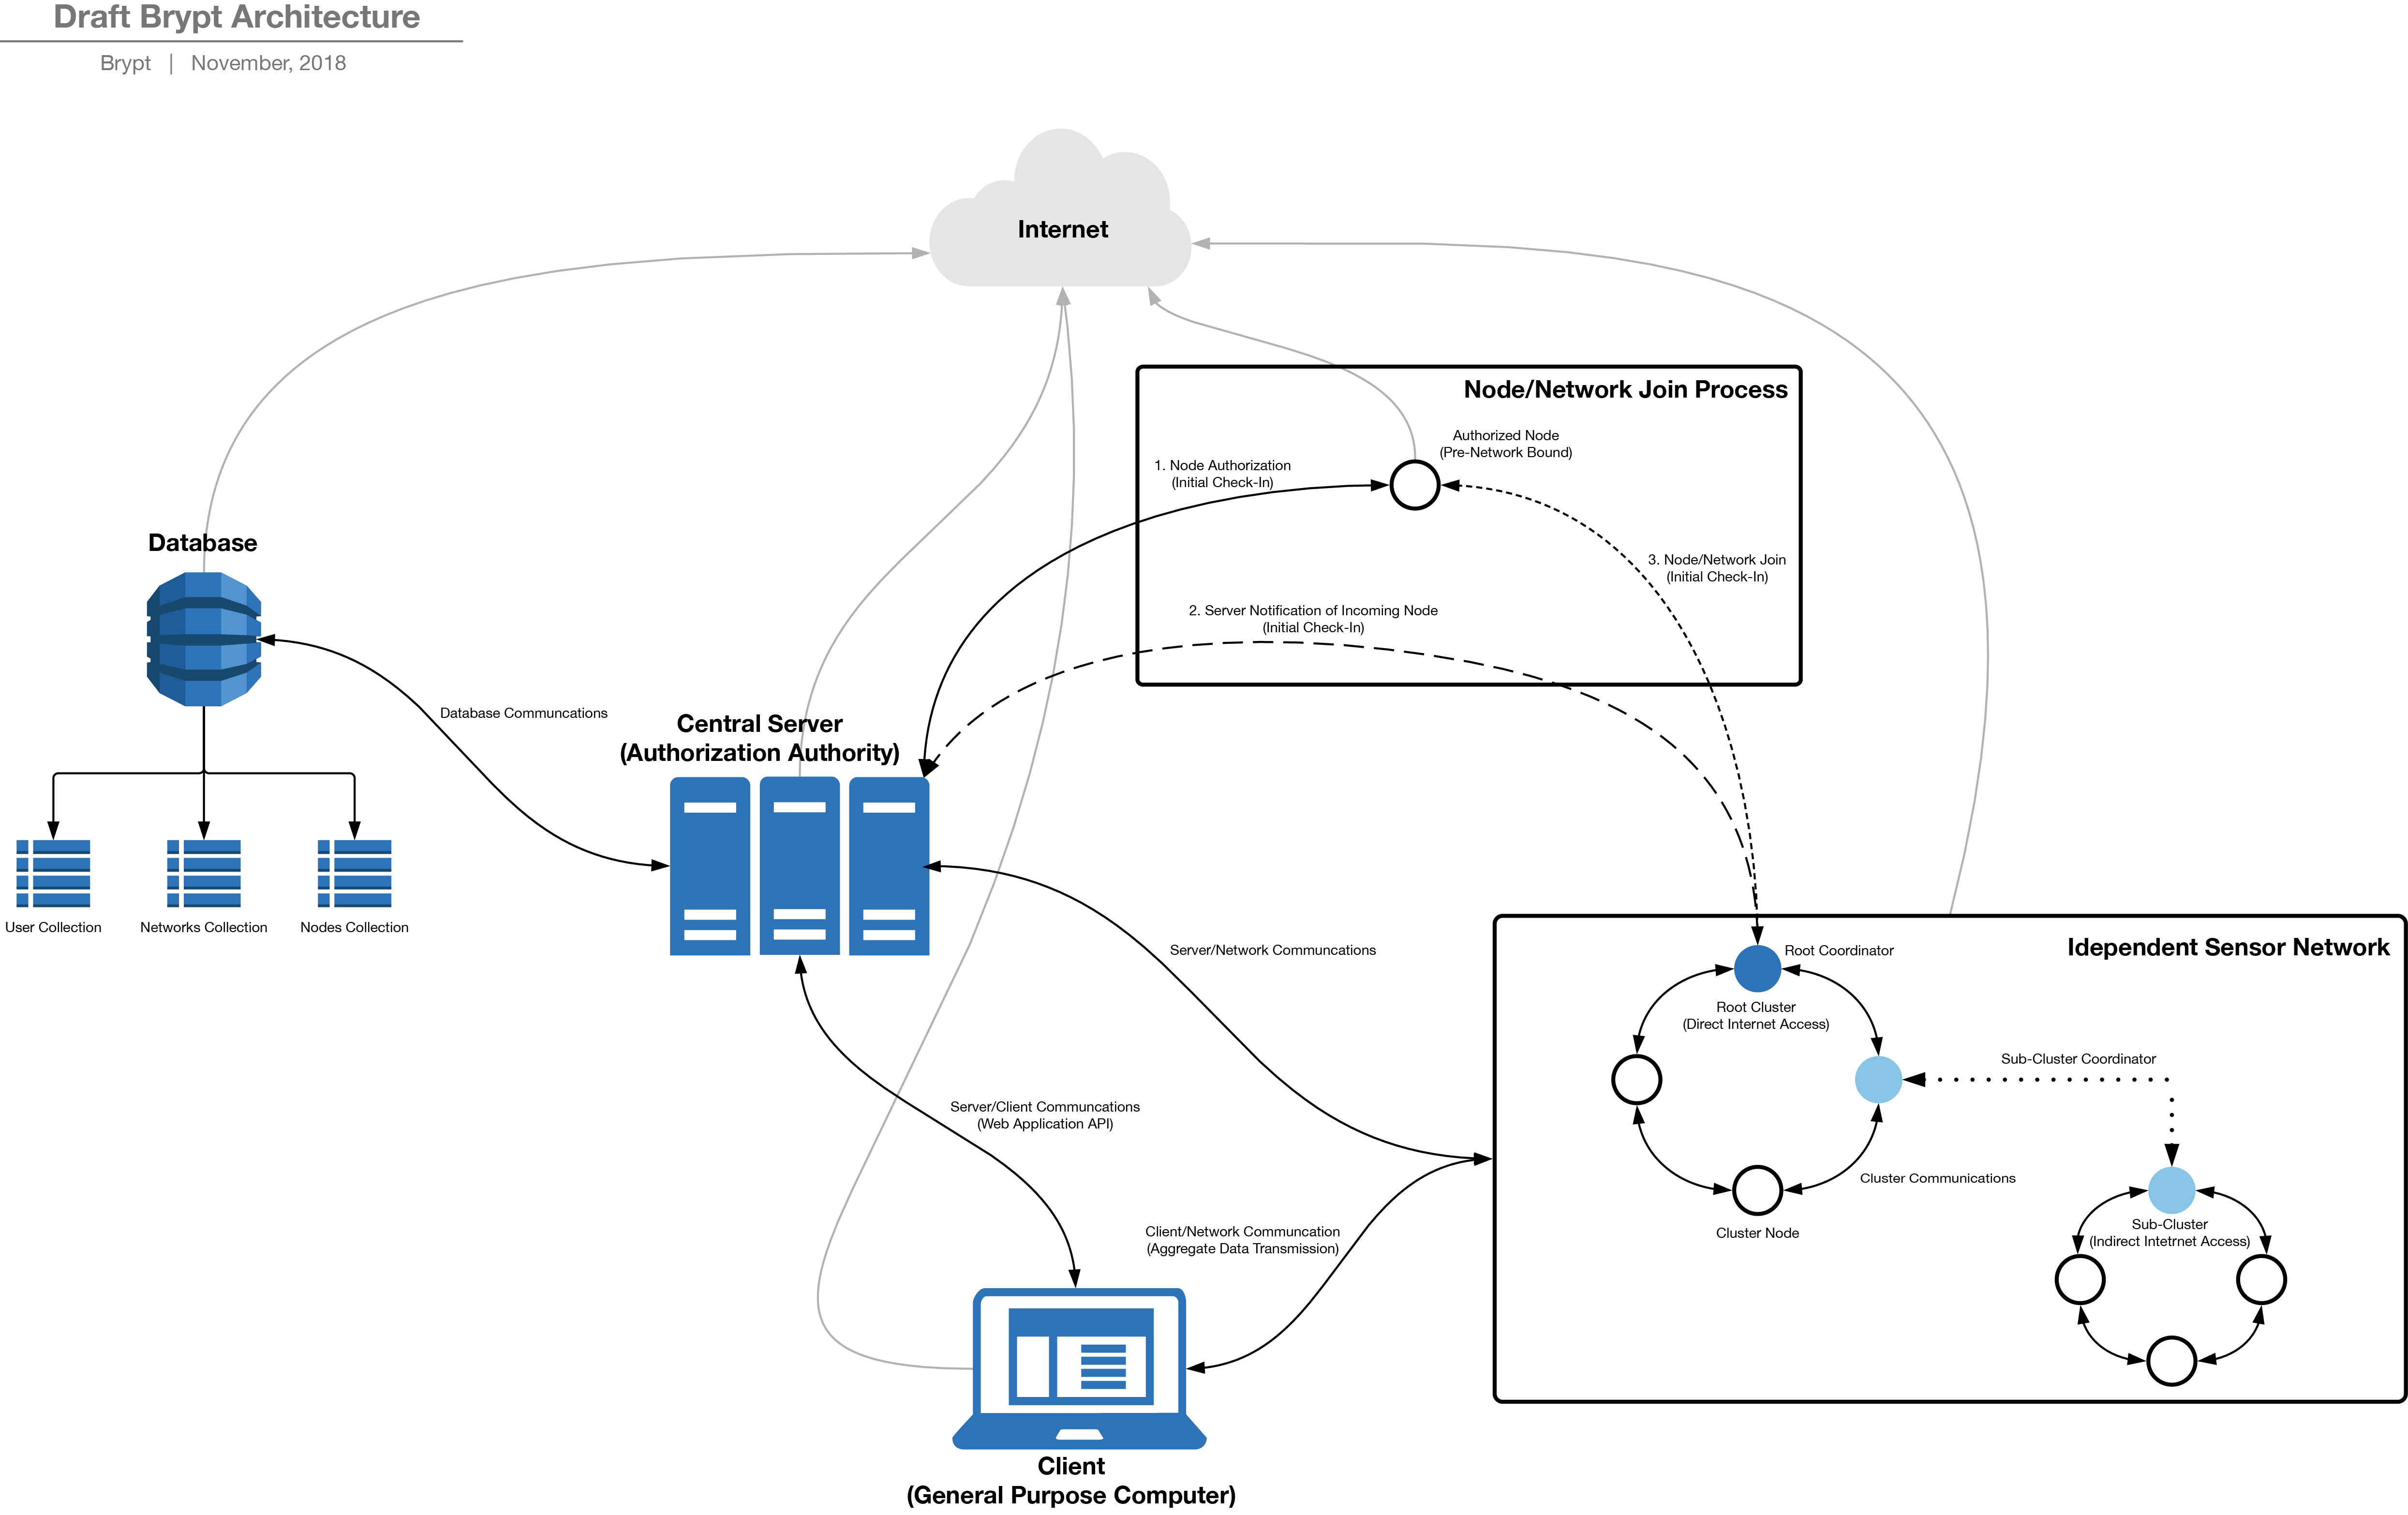
\includegraphics[width=1.5\linewidth]{Images/draft-brypt-architecture-medium.png}
    }
\end{turn}

\end{document}
